The aim of the superclustering procedure is to collect the majority of
the pixels belonging to a track which is long and can be split in
multiple parts in the clustering step described before.  Indeed, the
main limitation of \idbscan to follow a long track is mainly
originated by the non uniform energy release along the path length.
As can be clearly seen in Fig.~\ref{fig:basic_clusters} (right), or
even in the example of a raw image of an event with two long cosmic
rays in Fig.~\ref{fig:typicalimage1} (right), clusters with larger
energy release are followed by regions along the path with a lower or
even a zero release.  These local minima are sometimes as large, in
the 2D space, as the typical size of the $\epsilon$ parameter of
\dbscan~\cite{dbscan}. Despite the low electronic noise of the
\texttt{ORCA-Flash 4.0} camera sensor, the energy releases in these local
minima are similar in magnitude to the average single-pixel noise.

The \idbscan is limited in connecting the full length of an extended
path, because of two reasons. First, inflating $\epsilon$ parameter as
much as needed to cover the areas of local minima conflicts with the
need to reject noise around the cluster.  The basic cluster parameters
were optimized for the \lemon running conditions to collect most of
the signals with an energy as low as few keVs and to reject the
typical noise of $\approx 1$ photon per pixel. This avoids collecting
extra noise in the cluster, biasing the energy scale and worsening its
resolution, and keeps the rate of fake clusters at a negligible
level~\cite{iDBSCAN}.  Second, the iterative nature of the algorithm,
with different parameters for each iteration, each tuned for very
different intensity, makes it convenient and efficient for a
deposition of a fixed energy density (like the spots originating from
the \fe source), but not for the cases as in
Fig.~\ref{fig:basic_clusters} (right), where the same track is split
in several parts, some of them belonging to different iterations.
This requires a method that can continuously follow the pattern of the
track, profiting of the full resolution image, where the {\it
gradients} of the energy deposition along the track trajectory are
smaller than the ones in the transverse direction, but still give
information on the energy release pattern. Several existing algorithms
were tested to profit of this, but executing any of them on the full
$2048{\times}2048$ image is not manageable CPU-wise, due to the huge
pixel combinatorics.

Therefore, the procedure adopted for the final supercluster
reconstruction in the
\lemon detector starts from defining the \textit{interesting regions}
in the image that may contain pixels from an energy deposit. These are
identified by the basic cluster algorithm \idbscan previously
described, which is applied on the $512{\times}512$ reduced-resolution
image. In order to gather the peripheral pixels, especially along the
track trajectory where breaks into small basic clusters may have
happened, a window of $5{\times}5$ pixels is considered, around each
pixel belonging to a macro-pixel clustered in a basic cluster. A full
resolution image formed only by the interesting pixels passing the
simple initial filtering described in Sec.~\ref{sec:zerosuppression}
is created.  The gradients of the intensity $N_{ph}$ in such image are
computed pixel-by-pixel to look for the edge region where the image
turns from signal to noise-only:
%
\begin{equation}
\label{eq:gradient}
\vert\vert\nabla(N_{ph})\vert\vert =
\sqrt{\left(\frac{\partial N_{ph}}{\partial x}\right)^2
  +\left(\frac{\partial N_{ph}}{\partial y}\right)^2},
\end{equation}
%
while the gradient direction is given by:
\begin{equation}
  \label{eq:graddir}
  \theta = \tan^{-1}\left(\frac{\partial N_{ph}}{\partial y}/\frac{\partial N_{ph}}{\partial x}\right).
\end{equation}
%
In order to reduce the effect of the noise, which induces fluctuations
in the first derivatives of Eq.~\ref{eq:gradient}, a Gaussian filter
is applied, which smoothen the response by convolving the pixel
intensity with a Gaussian function, having as $\sigma$ the SD of the
intensities of all the pixels considered, and rejecting the ones
falling outside a 5$\sigma$ window.

The superclustering algorithm, applied on the filtered image, is an
application of the \textit{morphological geodesic active
contours}\cite{gac,mgac}, called \gac in the following.  This method
uses an active contour finding, widely used in computer vision, where
the boundary curve $\mathcal{C}$ of an object is detected by
minimizing the \textit{energy} $E$  associated to $\mathcal{C}$:
\begin{equation}
  \label{eq:gacenergy}
  E(\mathcal{C}) = \int_{0}^{1} g(N_{ph})(\mathcal{C}(p)) \cdot \vert\mathcal{C}_p\vert dp,
\end{equation}
where $ds=\vert\mathcal{C}_p\vert dp$ is the arc-length
parameterization of the curve in the 2D space, and $g$ is the stopping
edge function, which allows to select the boundary of the cluster.  In
the \gac method used for the \lemon images, the $g$ function is purely
geometrical, and uses the geodesics of the image, \ie, the local
minimal distance path joining points with the same light intensity
gradient. The function $g(N_{ph})$ is given by:
\begin{equation}
g(N_{ph}) = \frac{1}{\sqrt{1+\alpha\vert\nabla G_\sigma * N_{ph}\vert}},
\end{equation}
which is minimal in the edges of the image.  The $G_\sigma * N_{ph}$ is the
aforementioned $5\sigma$ Gaussian filter, and the parameter $\alpha$,
which regulates the strength of the filter, was tuned on
typical \lemon images to be $\alpha=100$.

This method was chosen because it allows to follow patterns that
may vary from convex to concave shape, eventually with kinks, \eg in
cases of $\delta$-ray emissions. To improve the shrinking of the
cluster boundary in the cases of tracks turning from concave to convex
along their trail, the \textit{balloon} force~\cite{mgac}, which is a
term added to Eq.~\ref{eq:gacenergy} to smooth the cluster contour, is
set to -1, in order to push the contour towards a border in the areas
where the gradient is too small. A number of 300 iterations is used to
evolve the supercluster contour.

The example track shown in Fig.~\ref{fig:basic_clusters} (right) after
the basic clustering step, is shown again in full resolution, zoomed
around the cluster, in Fig.~\ref{fig:super_clusters1} (left). The
output of the superclustering with the \gac algorithm is shown on the
right panel of the same figure. The splitting of the cluster,
happening at the basic clusters step, is recovered: the portions with
high and low density along the path of the energy release are joined
together. Other three examples of superclustered images are shown in
Fig.~\ref{fig:super_clusters2}, in runs without any artificial
radioactive source. The top left panel shows an example of a cosmic
ray track fully reconstructed by the \gac superclustering, which also
includes a $\delta$-ray in the middle of the track length. The top
right panel shows an example of curly track from a candidate of
natural radioactivity interaction; bottom panel shows an example where
both a cosmic ray and a curly track are present. In this case, the
extremes of the long and straight track are still split, but this is
much rarer than after the basic clustering, and it happens when the
local minima along the trajectories are compatible with noise-only
for more than $\approx$1\unit{cm}.
%
\begin{figure}[ht]
  \begin{center}
     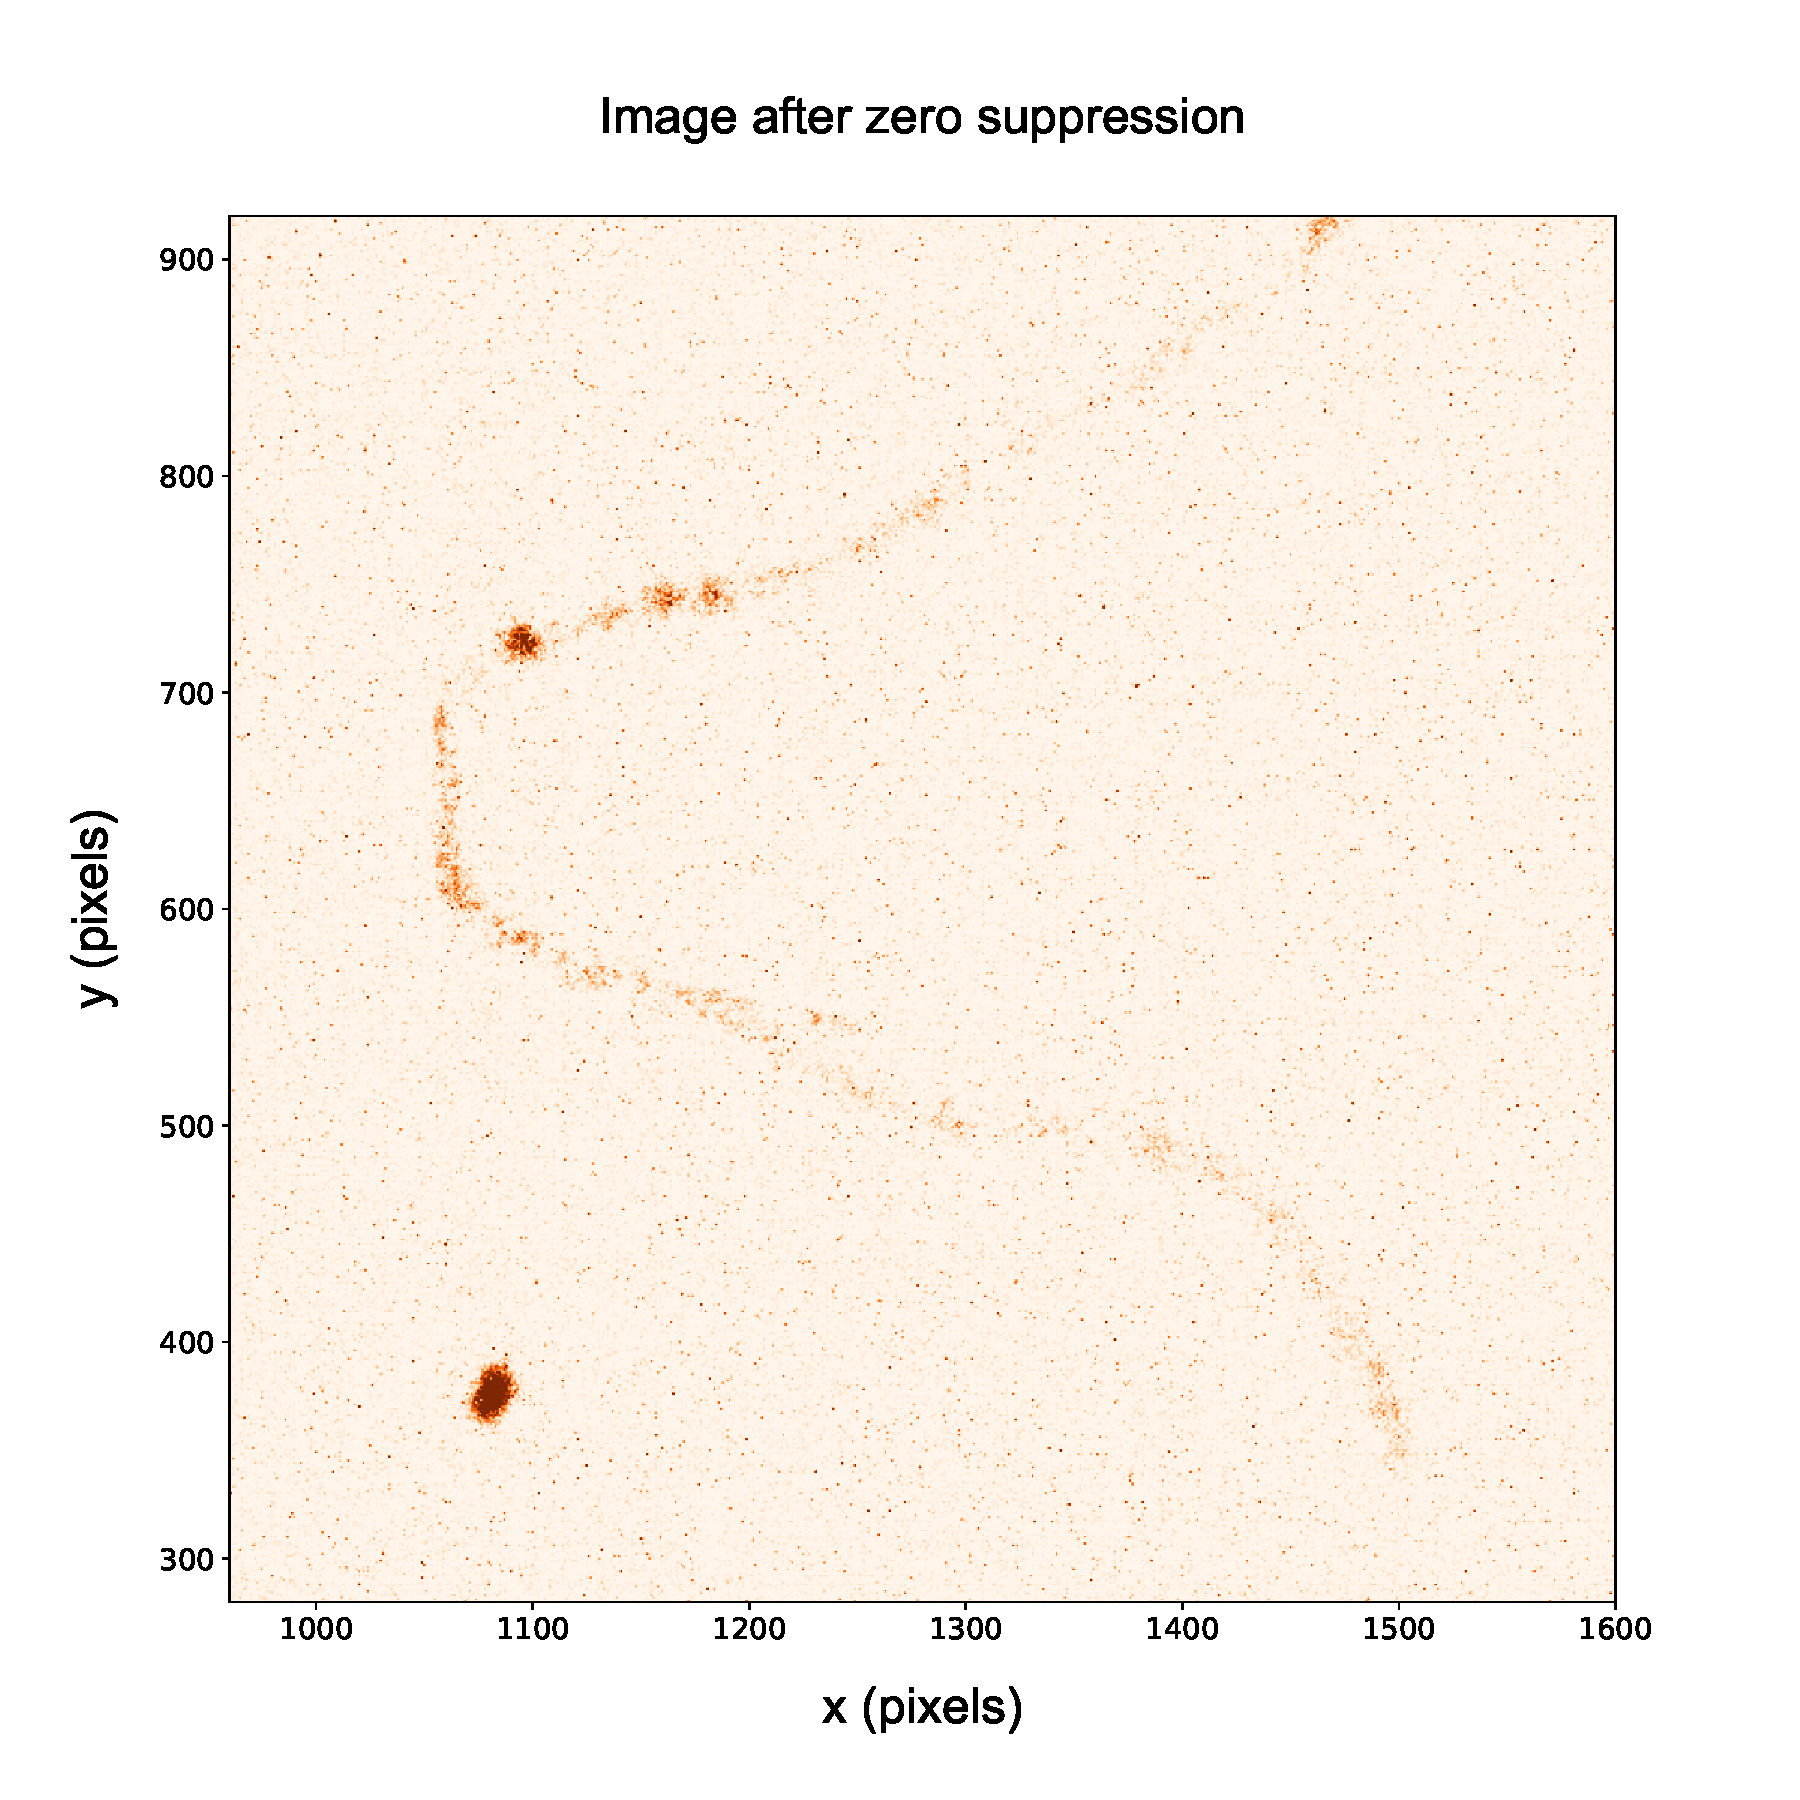
\includegraphics[width=0.49\linewidth]{figures/pic_run02317_ev8_oriIma_paper_zoom}
      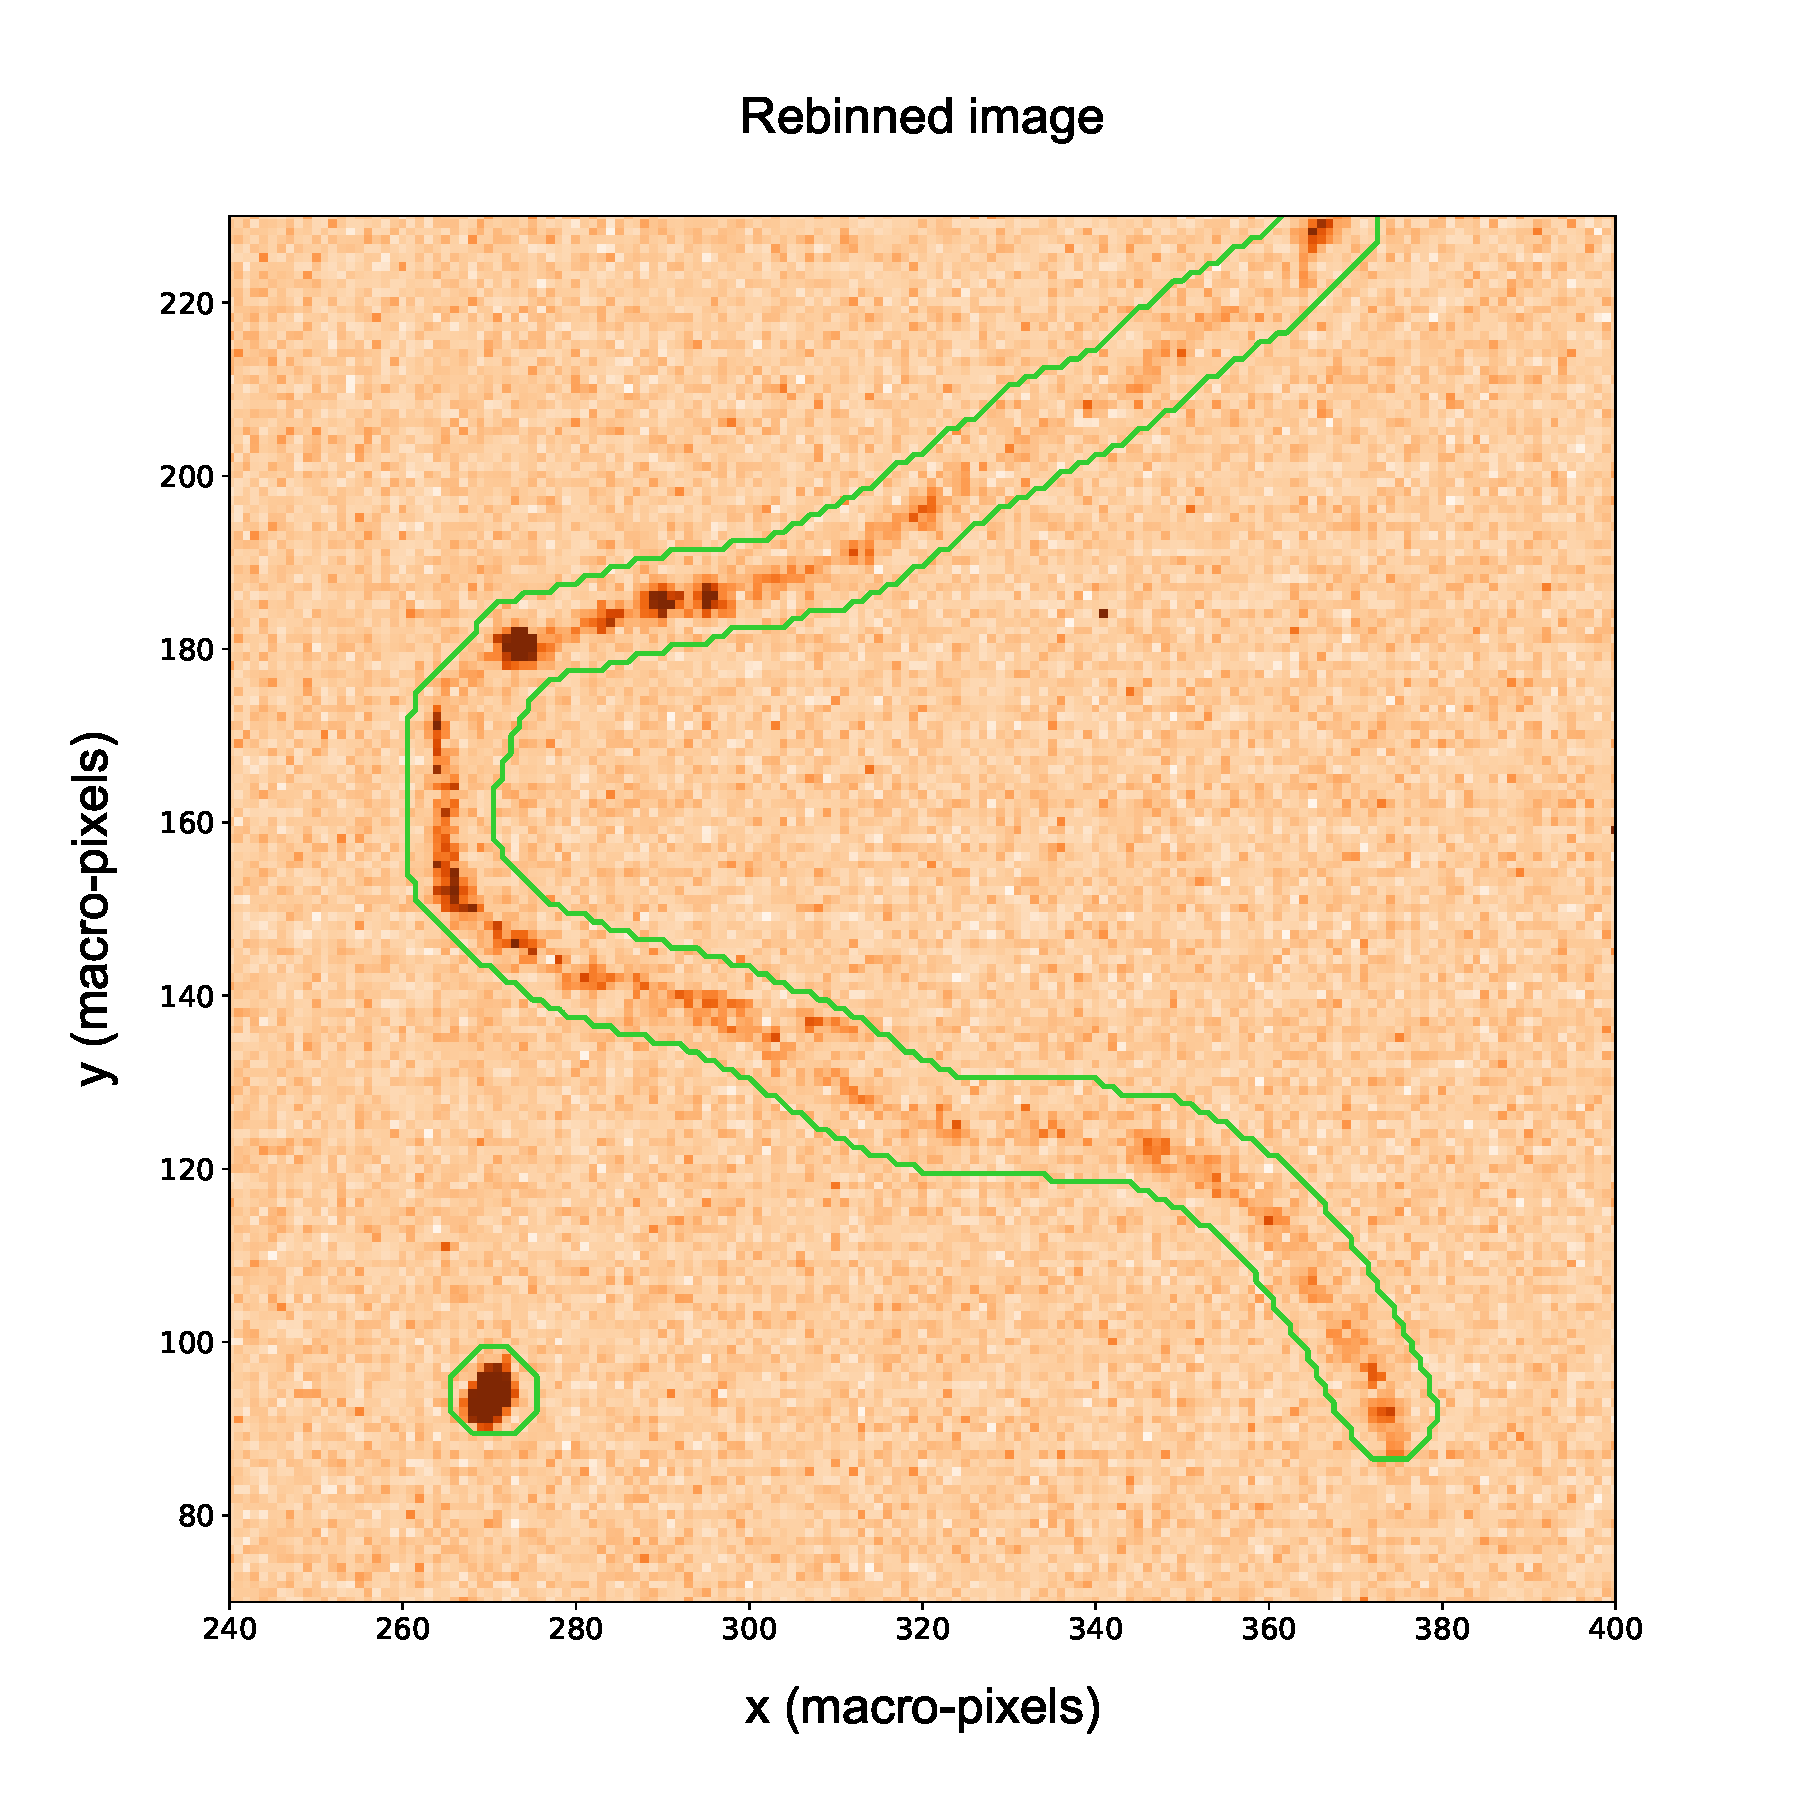
\includegraphics[width=0.49\linewidth]{figures/pic_run02317_ev8_sc_3D_paper}
      \caption{Left: zoom on the full-resolution image of a track
        candidate in a run with the \ambe radioactive source. Right:
        output of the superclustering on the rebinned image. The
        continuous line represents the approximate contour of the
        reconstructed supercluster. \label{fig:super_clusters1}}
  \end{center}
\end{figure}
%
\begin{figure}[ht]
  \begin{center}
     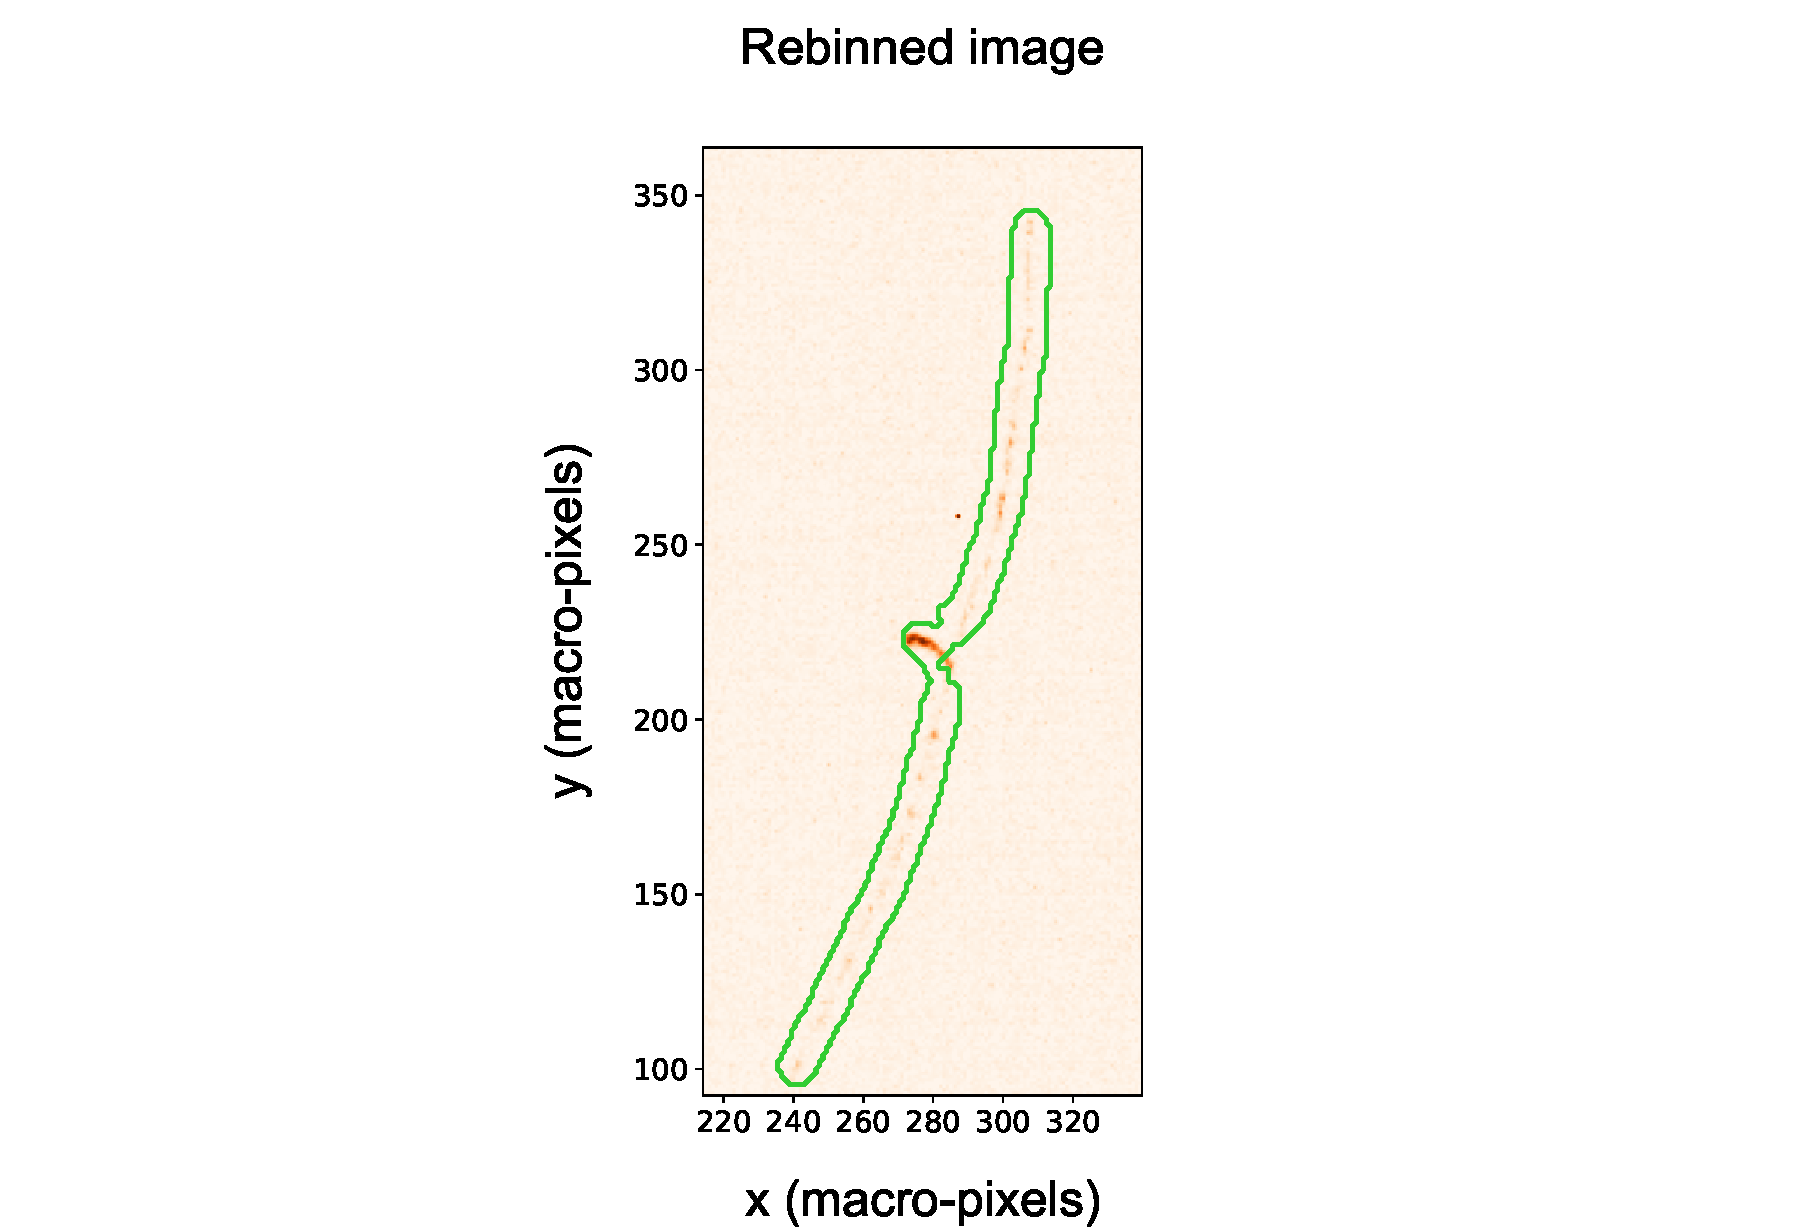
\includegraphics[width=0.49\linewidth]{figures/pic_run02156_ev49_sc_3D_paper}
     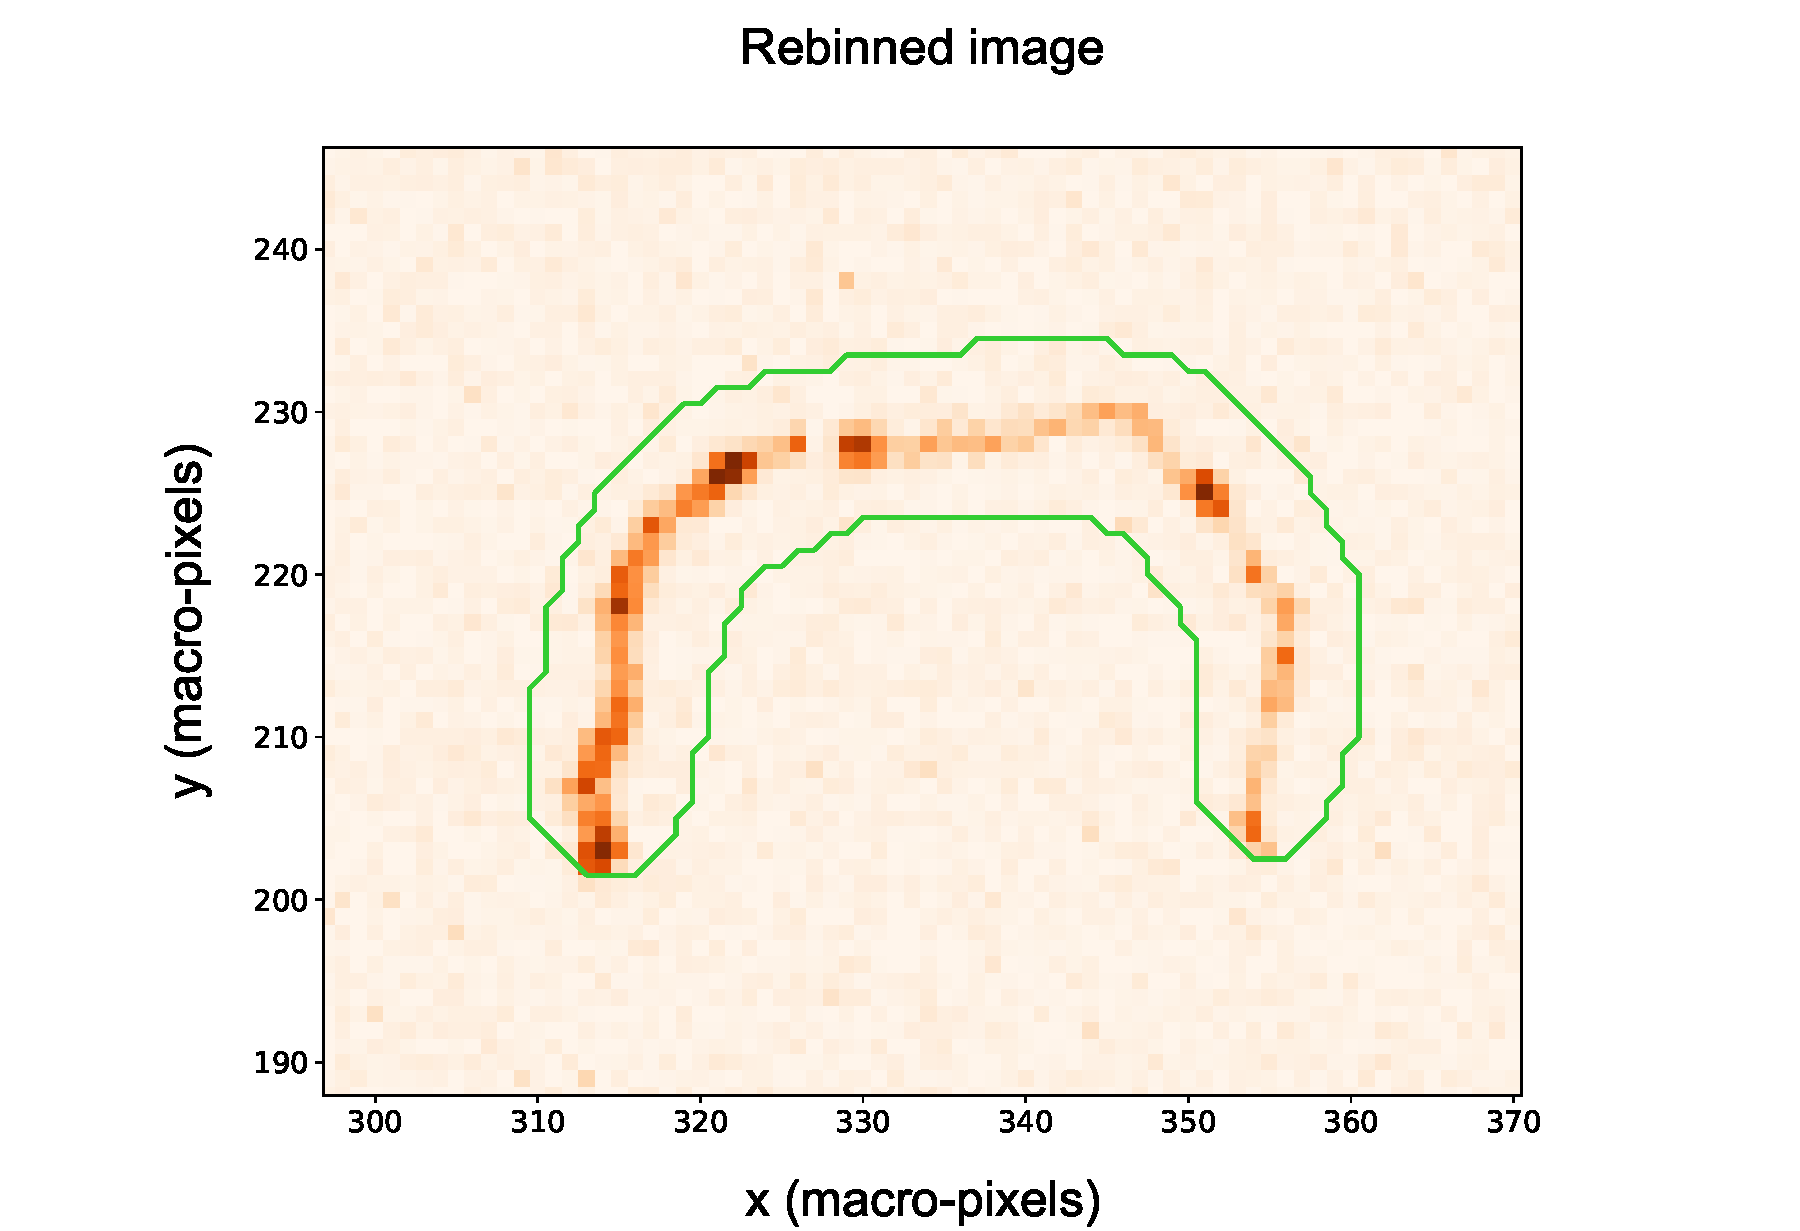
\includegraphics[width=0.49\linewidth]{figures/pic_run02156_ev641_sc_3D_paper} \\
     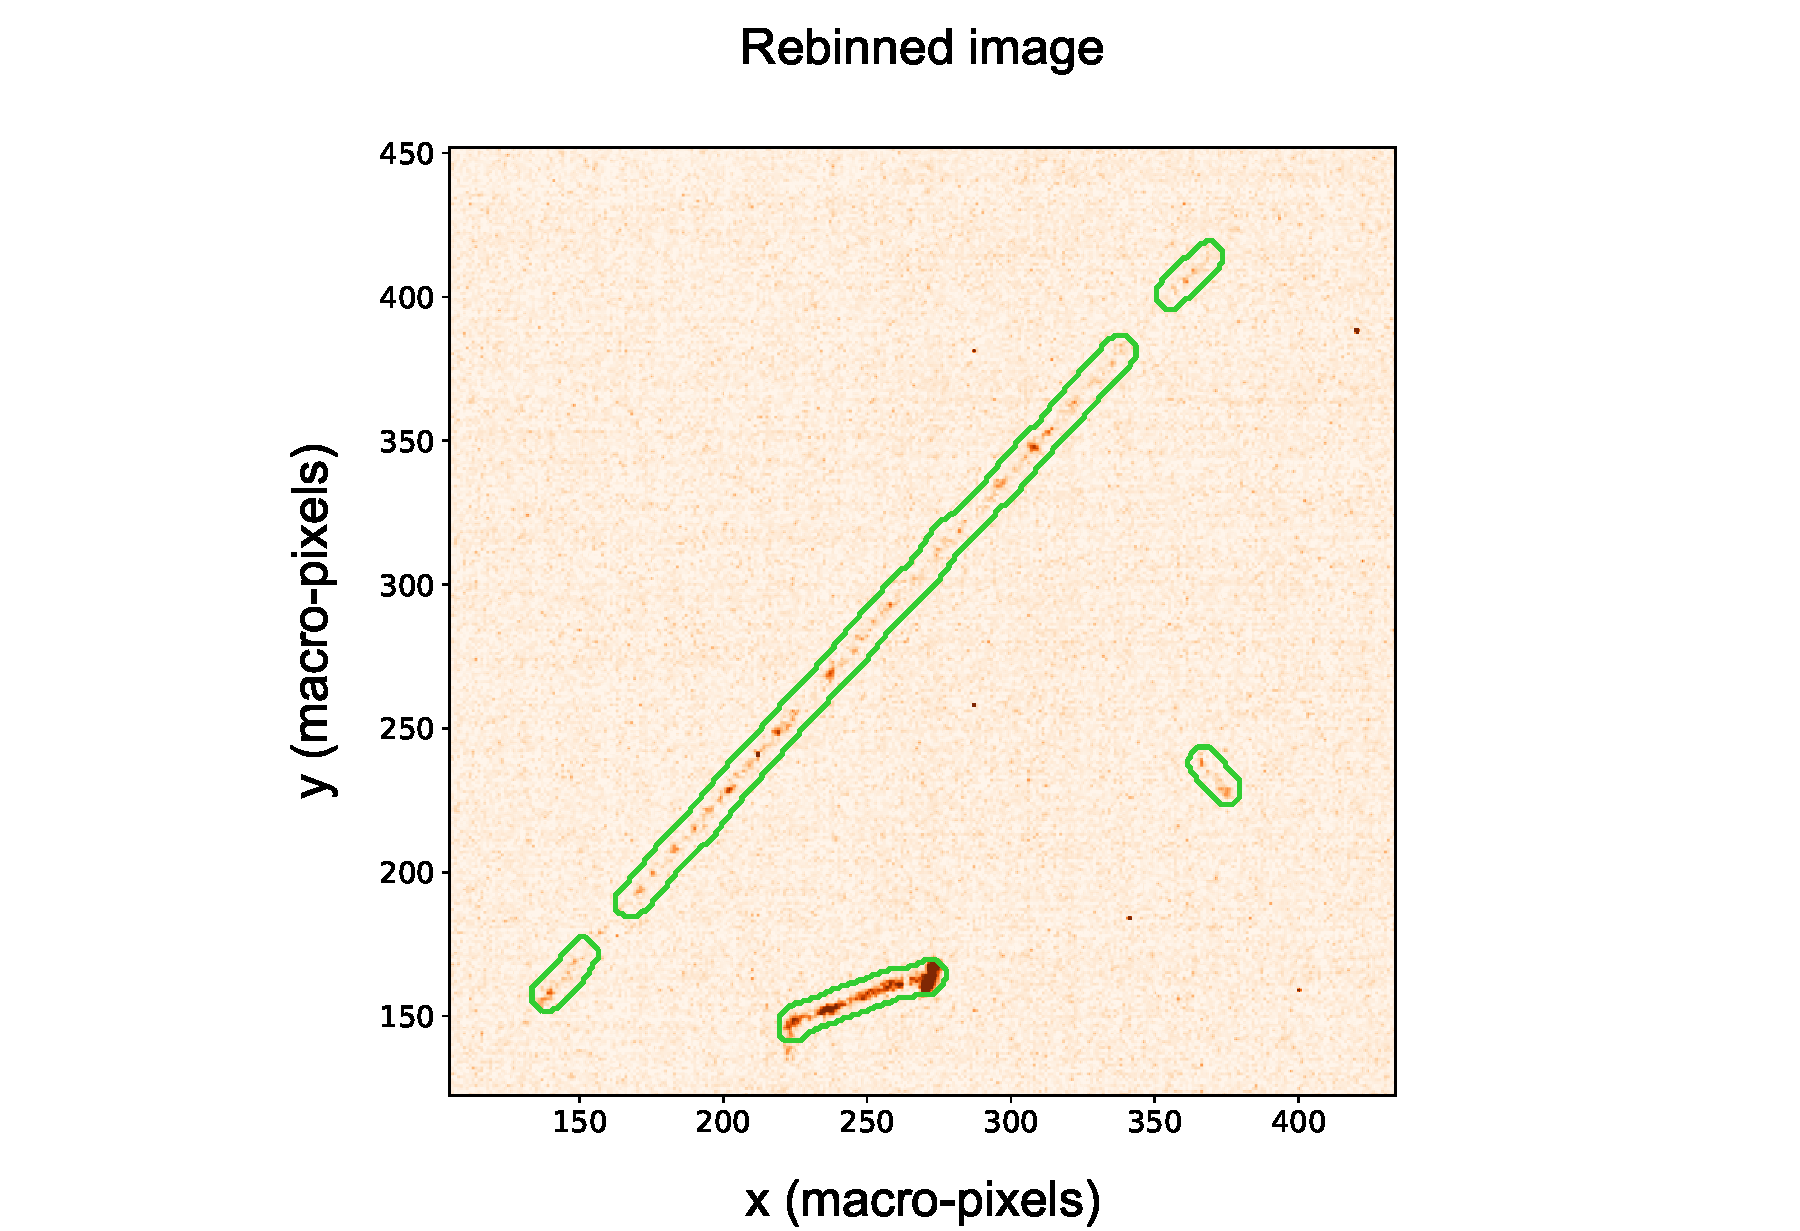
\includegraphics[width=0.6\linewidth]{figures/pic_run02156_ev631_sc_3D_paper}

     \caption{Superclusters reconstructed in a run without artificial
       radioactive sources. The continuous lines represent the
       approximate contours of the reconstructed superclusters. Top
       left: cosmic ray track fully reconstructed by the \gac
       superclustering. A $\delta$-ray is included in the
       supercluster. Top right: curly track from a candidate of
       natural radioactivity interaction. Bottom: a cosmic ray with
       the extremes not joined to the main track, plus a curly track
       from natural radioactivity. \label{fig:super_clusters2}}
       
  \end{center}
\end{figure}
